\documentclass{article}
\usepackage{pgfplots}
\pgfplotsset{compat=1.18}

\begin{document}

\begin{figure}[ht]
    \centering
    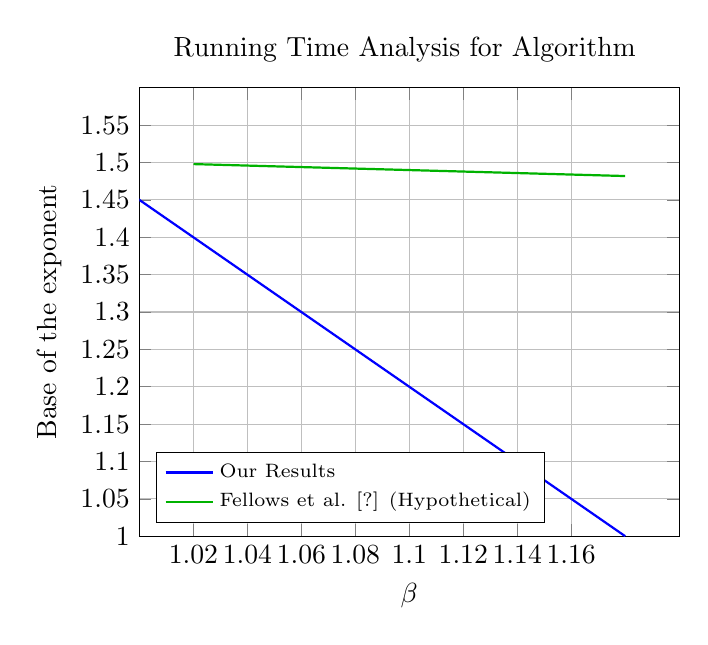
\begin{tikzpicture}
        \begin{axis}[
            xlabel = {$\beta$},
            ylabel = {Base of the exponent},
            xmin=1, xmax=1.2,
            ymin=1, ymax=1.6,
            xtick={1.02, 1.04, 1.06, 1.08, 1.1, ..., 1.18},
            ytick={1, 1.05, 1.1, 1.15, 1.2, ..., 1.6},
            grid=major,
            legend pos=south west,
            title style={align=center},
            title={Running Time Analysis for Algorithm $\vcmaxdegthree$},
            legend cell align={left},
            legend style={draw=black, fill=white, font=\scriptsize},
        ]
            \addplot[blue, thick] coordinates {
                (1.18, 1)
                (1.16, 1.05)
                (1.14, 1.1)
                (1.12, 1.15)
                (1.10, 1.2)
                (1.08, 1.25)
                (1.06, 1.3)
                (1.04, 1.35)
                (1.02, 1.4)
                (1, 1.45)
                (0.98, 1.5)
                (0.96, 1.55)
                (0.94, 1.6)
            };
            \addlegendentry{Our Results}
            
            \addplot[green!70!black, thick,domain=1.18:1.02,samples=100] expression {1.5 - 0.1 * (x - 1)};
            \addlegendentry{Fellows et al. [?] (Hypothetical)}
        \end{axis}
    \end{tikzpicture}
    \caption{Comparison of Running Times between Our Algorithm and Hypothetical Lower Bound (\cite{fellows2006parameterized})}
    \label{fig:running_time_comparison}
\end{figure}

\end{document}